\section{Modellierung mit Unity}

\subsection{Gelände}
\begin{figure}[h]
\centering
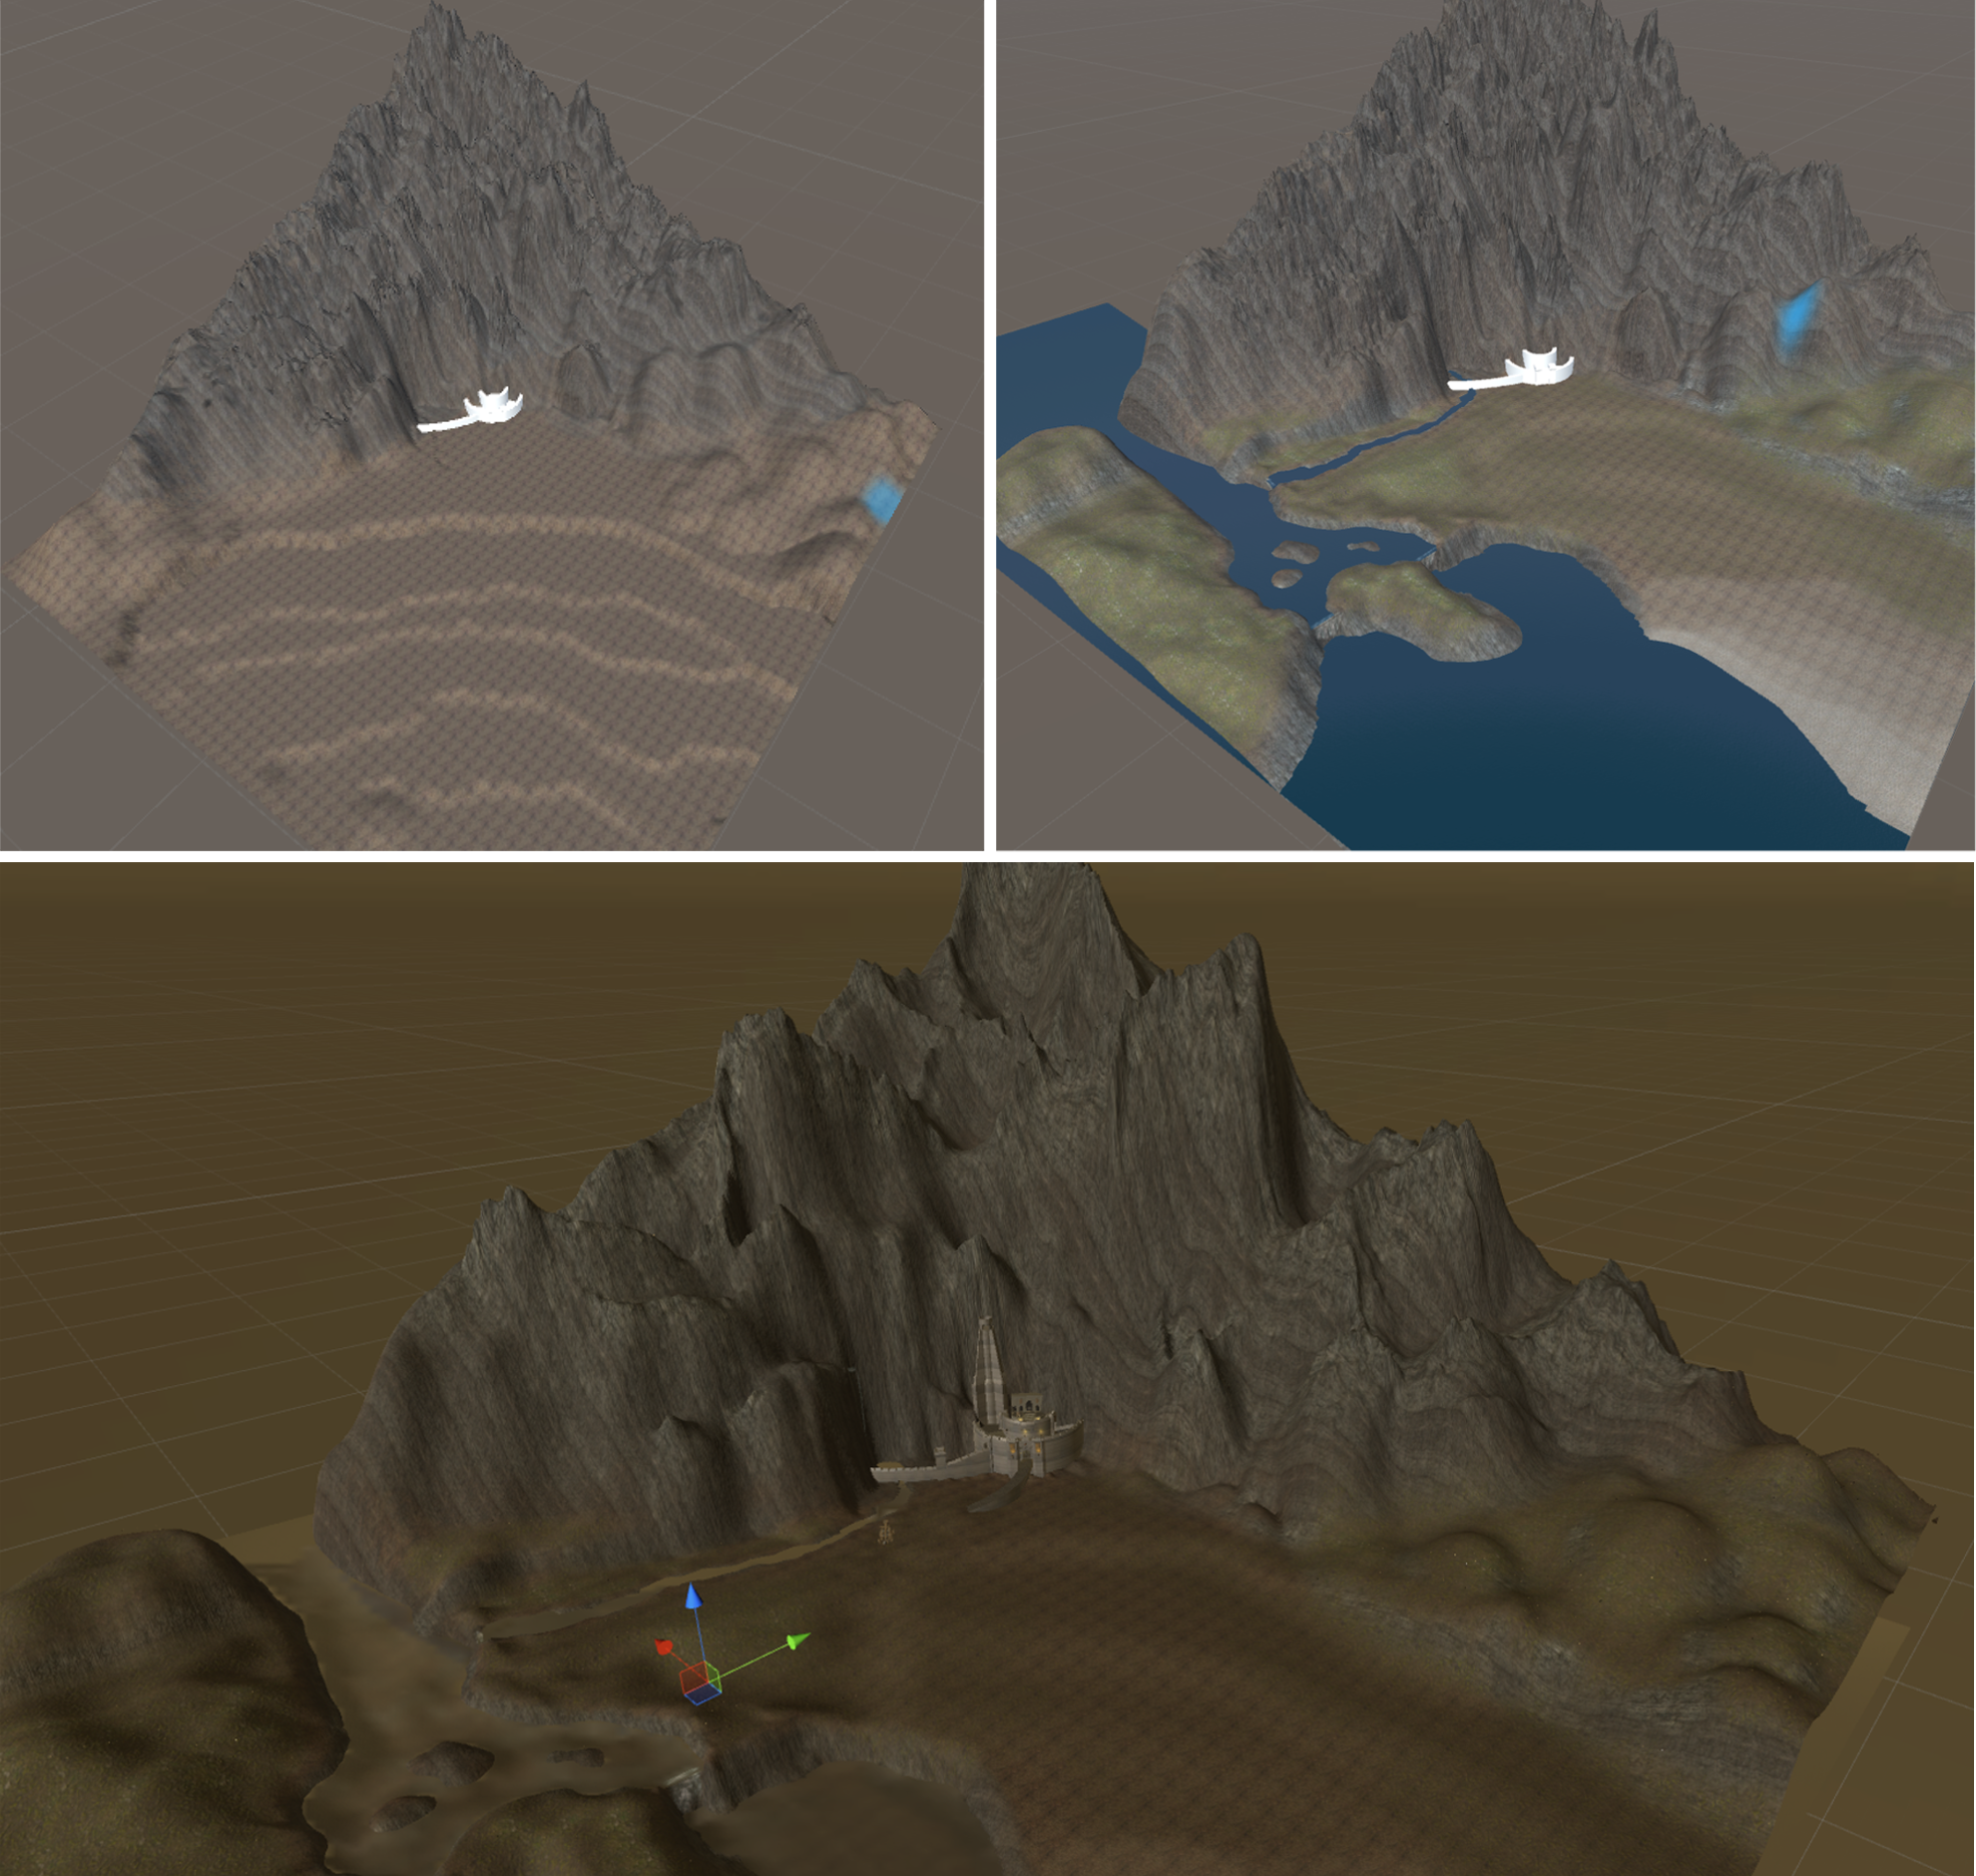
\includegraphics[width=0.95\linewidth]{Abbildungen/Unity/TerrainProgress}
\caption{Entwicklungsschritte des Geländes}
\label{fig:TerrainProgress}
\end{figure}

\begin{wrapfigure}[8]{r}{0.5\textwidth}
	\vspace{-20pt}
	\begin{center}
		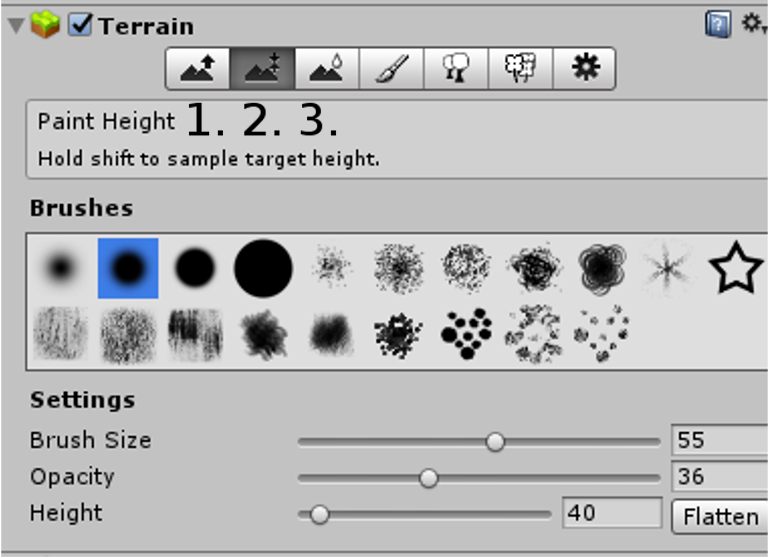
\includegraphics[width=0.45\textwidth]{Abbildungen/Unity/TerrainTool}
	\end{center}
	\caption{Terrain Werkzeuge}
	\label{fig:TerrainWerkzeuge}
\end{wrapfigure}

Die Abb. \ref{fig:TerrainProgress} zeigt verschieden Zwischenstände in der Gestaltung des Geländes. Die genutzten Werkzeuge sind in Abb. \ref{fig:TerrainWerkzeuge}, namentlich \textit{Raise/Lower} (1.), \textit{Paint Height} (2.) und \textit{Smooth Height} (3.), zu sehen. In allen drei Werkzeugen stehen verschieden Einstellungen für die Weite und Deckkraft des Pinsels zur Verfügung. Das Werkzeug \textit{Raise/Lower} ist besonders empfindlich und deshalb sollten für dieses nur niedrige Deckkraftwerte eingestellt werden.

%\newpage
Um ein gutes Größenverhältnis zwischen Burg und Gelände zu erreichen wurden die Maße des Terrains auf 500*500*600 festgelegt. Die Starthöhe des Geländes wurde mittels \textit{Paint Height} und \textit{Flatten} auf 50m gesetzt und von diesem Punkt heraus wurden die anderen Teile Stück für Stück herausgearbeitet. Mittel der Wahl war eine Kombination aus \textit{Paint Height} und \textit{Smooth Height}, gut zu sehen links oben in Abb. \ref{fig:TerrainProgress}. Zuerst wurde terrassenförmig die Höhe herausgearbeitet und danach wieder geglättet, um für fließende Übergänge zu sorgen. Das Gebirge im Hintergrund wurde größtenteils mit \textit{Raise/Lower} gestaltet. Es unterlag allerdings im Designprozess vielen Änderungen, da die Wirkung aus der Ego-Perspektive und das Zusammenspiel mit der Festung nicht optimal war. Im unteren Teil der Abb. \ref{fig:TerrainProgress} ist der finale Zustand des Geländes zu sehen.

\subsection{Texturierung}
\begin{figure}[h]
	\centering
	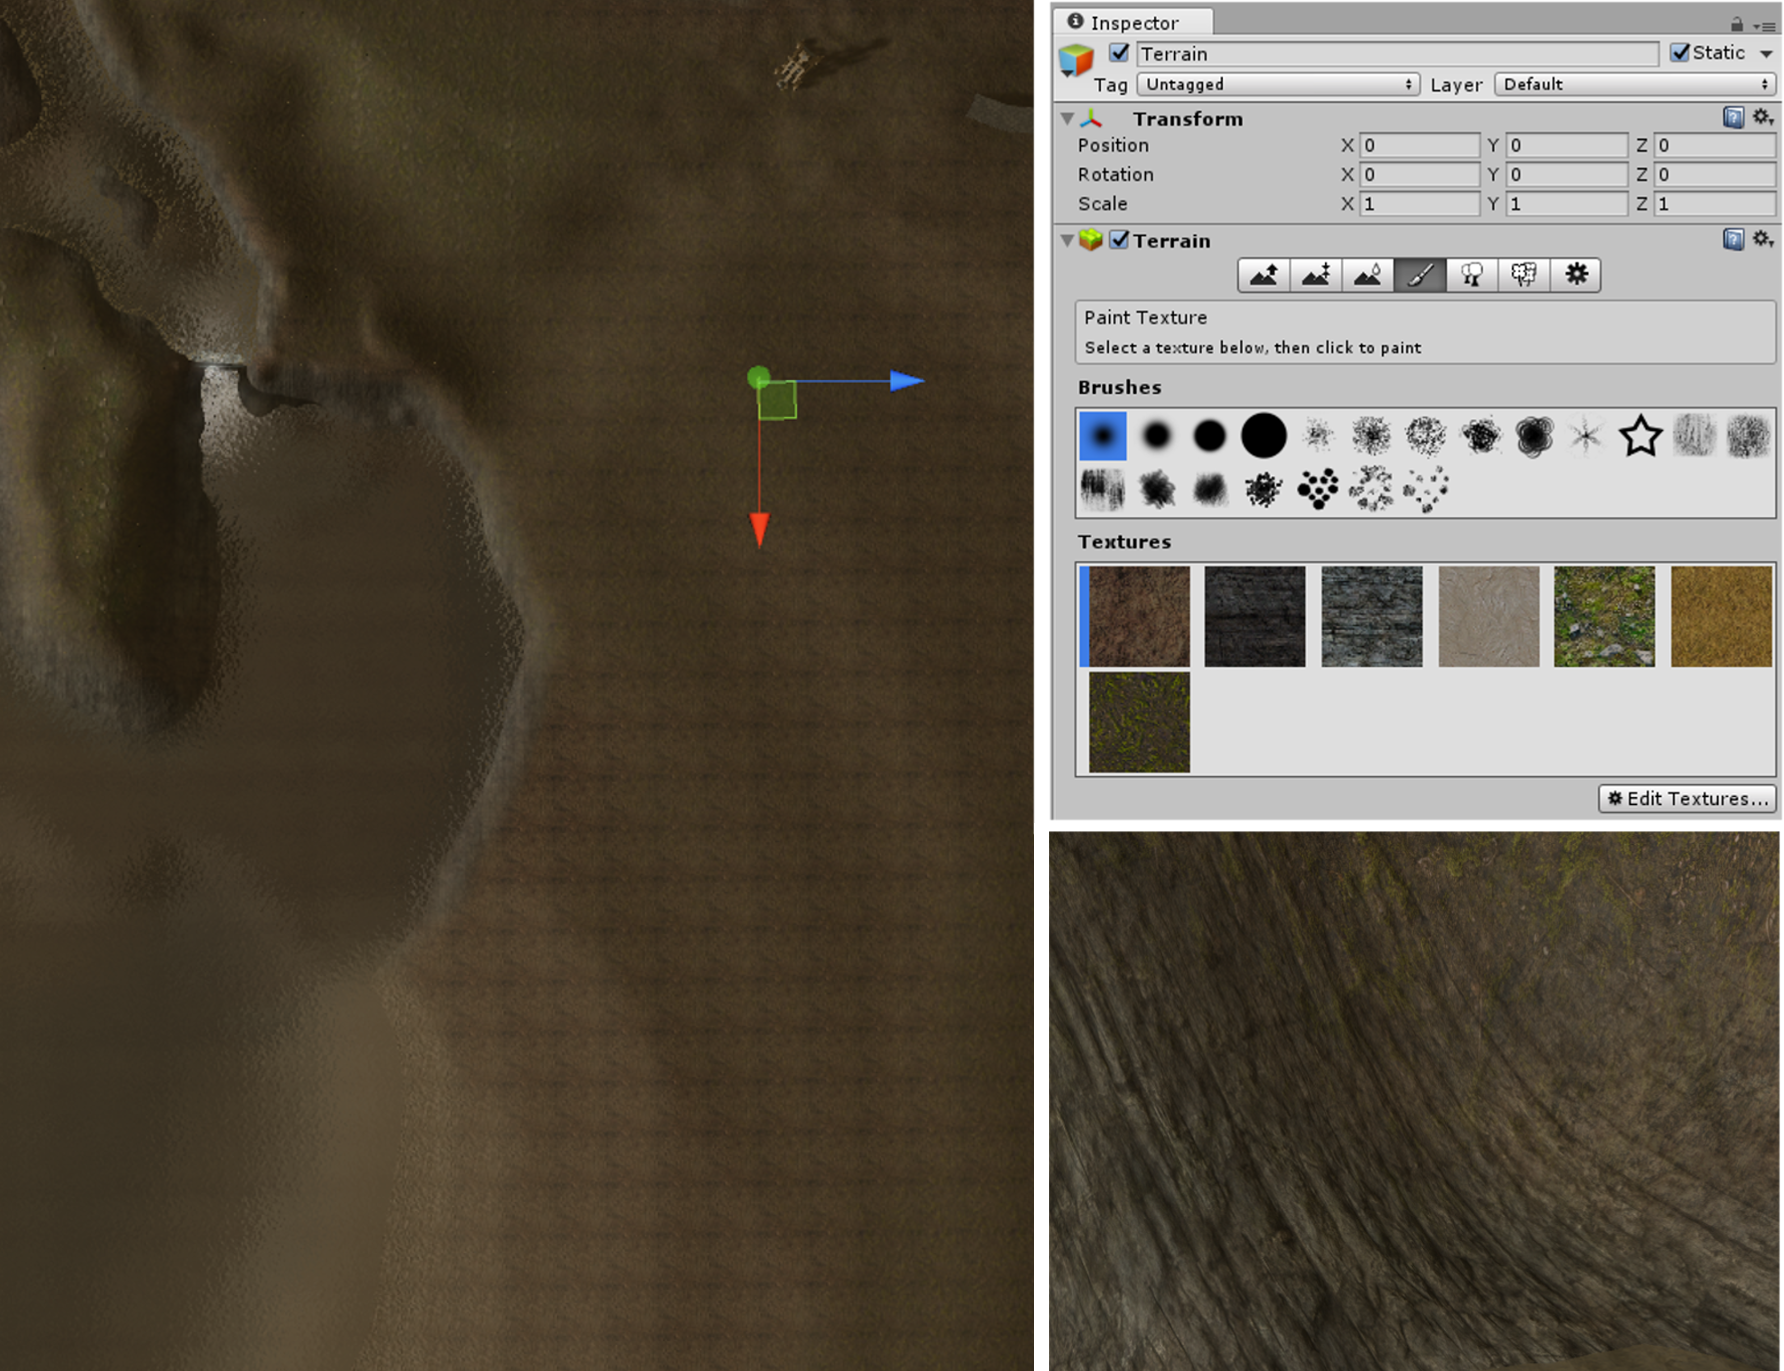
\includegraphics[width=0.95\linewidth]{Abbildungen/Unity/Texture}
	\caption{Wasserebenen und exemplarische Einstellungen}
	\label{fig:Textures}
\end{figure}

Das Gelände mit Texturen zu versehen ist in Unity denkbar einfach und selbsterklärend. Die Abb. \ref{fig:Textures} zeigt das Werkzeug zum Bemalen des Geländes. Es ist vergleichbar mit gängigen Grafikprogrammen. Über die Schaltfläche \textit{Edit Textures} können neue Texturen hinzugefügt werden. Danach stehen diese zur Verfügung und werden mithilfe des Pinsels auf das Gelände aufgetragen. Links in der Abbildung sind die weichen Übergänge von Sand, Erde, Gras und Fels sehen. Diese werden durch geringe Deckkrafteinstellungen und mehrmaliges Auftragen der Texturen erreicht. Eher schroffe Übergänge, unten rechts zu sehen, können durch höhere Deckkraft- und Stärkewerte (\textit{Target Strength}) erzielt werden. Die verwendeten Texturen stammen aus dem Assetstore.

\subsection{Wasser und Wasserfälle}
\subsubsection{Wasser}
In der Szene werden für die Darstellung von Flüssen und Ozean drei Wasserebenen benutzt. Als Asset wird das Standardwasser \textit{WaterProTime} aus Unity verwendet. In Abb. \ref{fig:Water} sind die drei Ebenen (1. kleiner Fluss, 2. großer Fluss und 3. Ozean) zu sehen. Zur Visualisierung des Gefälles wurden die Wasserebenen der Flüsse, im Bild rechts für Ebene 2. zu sehen, geneigt. Schwierigkeiten bei der Verwendung mehrerer Wasserebenen ergeben sich beim Übergang zwischen Zweien und der Wechselwirkung mit dem Gelände. Die Übergänge können beispielsweise durch die Verwendung von Wasserfällen kaschiert werden. 

\begin{figure}[h]
	\centering
	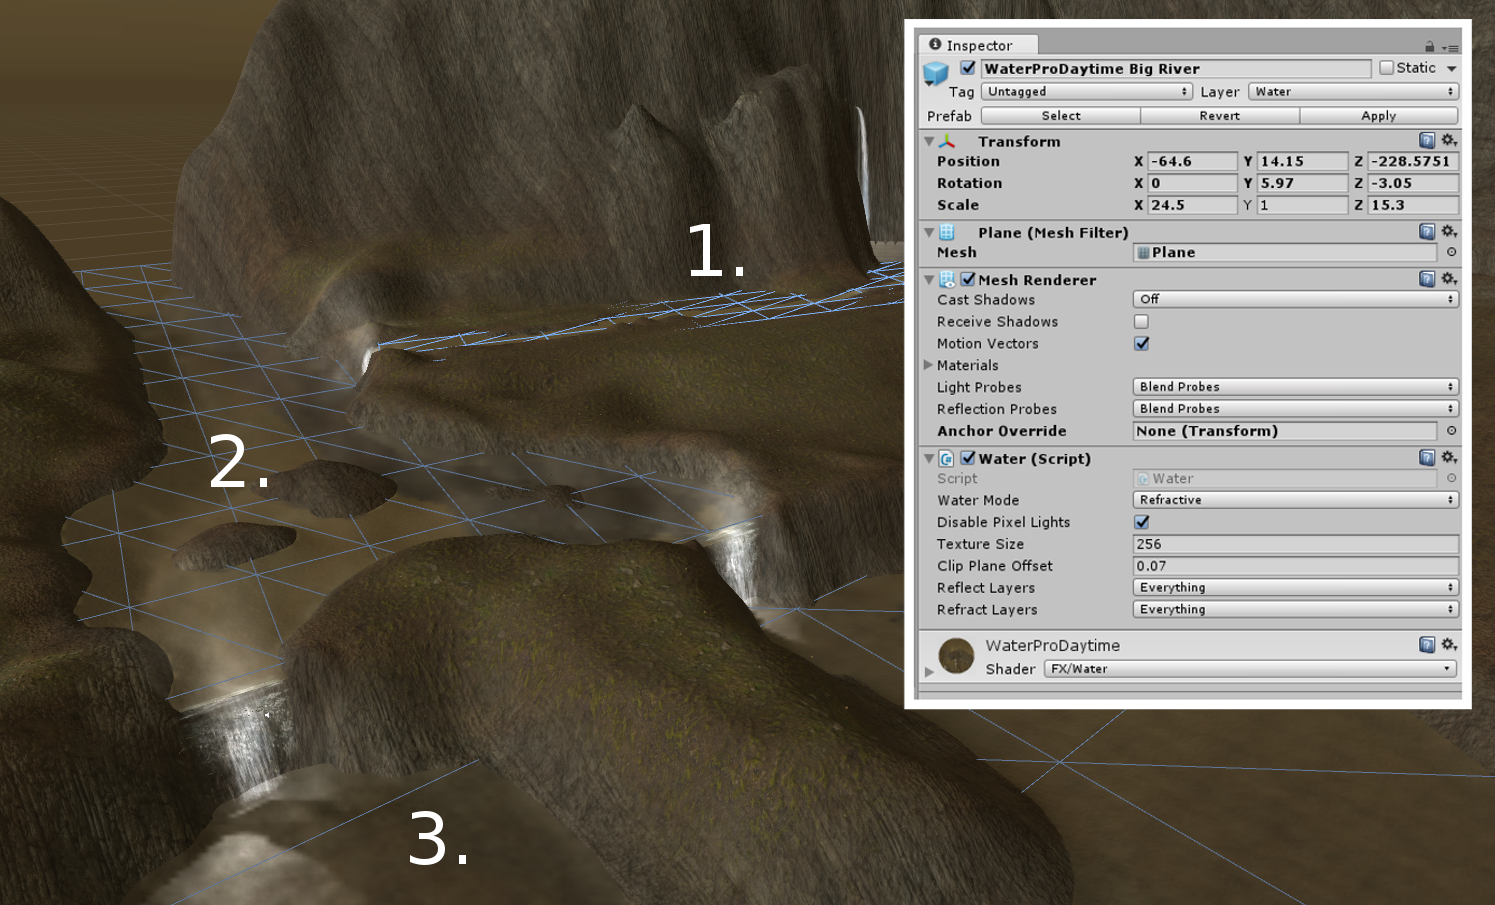
\includegraphics[width=0.95\linewidth]{Abbildungen/Unity/Water}
	\caption{Wasserebenen und exemplarische Einstellungen}
	\label{fig:Water}
\end{figure}

\subsubsection{Wasserfälle}
\begin{wrapfigure}{r}{0.5\textwidth}
	%\vspace{-20pt}
	\begin{center}
		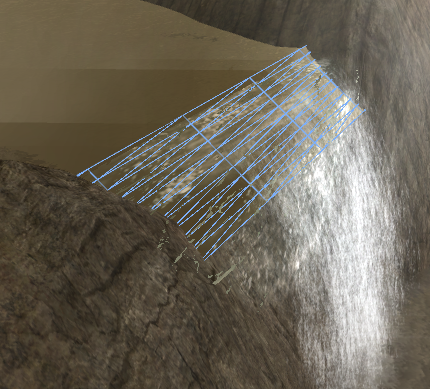
\includegraphics[width=0.45\textwidth]{Abbildungen/Unity/Waterfall}
	\end{center}
	\caption{Wasserfall}
	\label{fig:Waterfall}
\end{wrapfigure}

Trotz der Neigung der Flüsse konnten die Höhenunterschiede zwischen den Wasserebenen nicht ausgeglichen werden. Dadurch wurde es notwendig Wasserfälle in die Szene einzufügen. Diese stammen aus dem Assetstore und wurden für die Zwecke des Projektes angepasst. Die Abb. \ref{fig:Waterfall} zeigt den Übergang zwischen dem kleinen und großen Fluss. Um den harten Wechsel von Wasserebene zu Wasserfall abzuschwächen, war es nötig eine kleine abgeschrägte Ebene passgenau einzufügen. Ebenso mussten die seitlichen Ränder mit dem Terrainwerkzeug verdeckt werden. Diese Technik wurde auch bei den beiden anderen Wasserfällen vom großen Fluss zum Ozean angewendet.

\subsection{Animationen}
\subsubsection{Unity Animationen}
\begin{figure}[h]
	\centering
	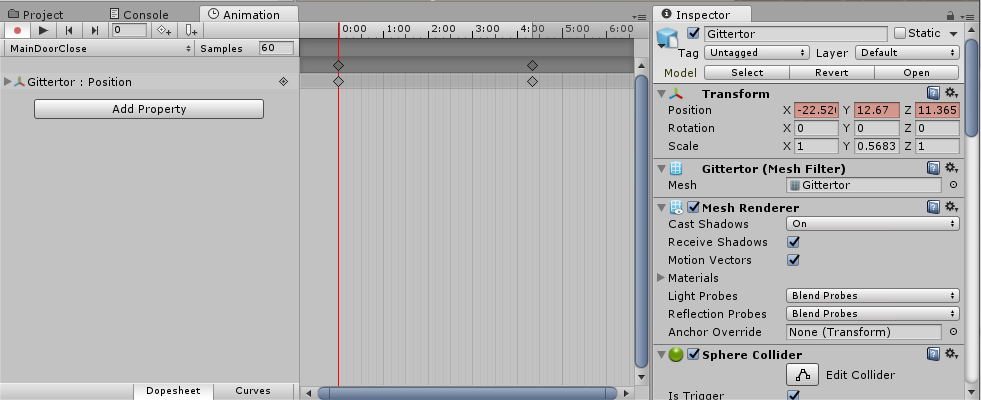
\includegraphics[width=0.95\linewidth]{Abbildungen/Unity/UnityAnim2}
	\caption{Erstellung von Animationen in Unity}
	\label{fig:unityAnim}
\end{figure}

Einfache Animationen, wie das Öffnen eines Burgtores können in Unity schnell und unkompliziert erstellt werden. In Abb. \ref{fig:unityAnim} ist das Werkzeug zur Erstellung von Animationen zu sehen. Im mittleren Teil sieht man die Keyframes und rechts die dazugehörigen \textit{Transform}-Werte. In unserem Fall des Burgtores wird das Schließen über zwei Keyframes mit unterschiedlichen Y-Werten definiert. Die so erstellten Animation stehen später im Animation Controller zur Verfügung.

\subsubsection{3d Studio Max Animation}

\begin{wrapfigure}{r}{0.6\textwidth}
	%\vspace{-20pt}
	\begin{center}
		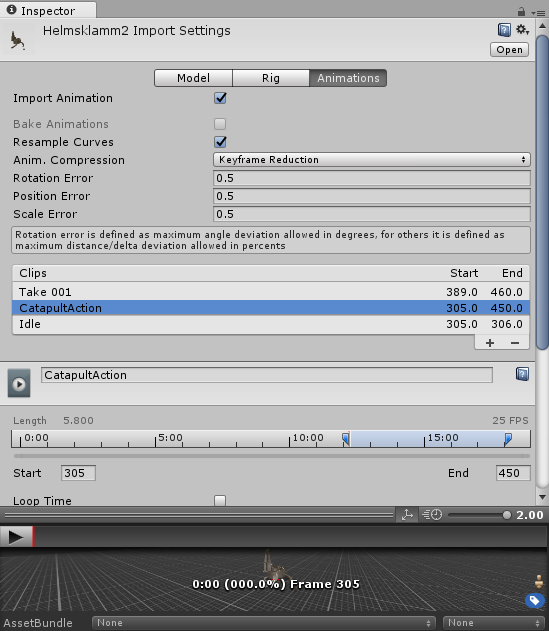
\includegraphics[width=0.55\textwidth]{Abbildungen/Unity/3dsAnim}
	\end{center}
	\caption{Animation aus 3d Studio Max}
	\label{fig:3dsAnim}
\end{wrapfigure}

\blindtext

\subsubsection{Animation Controller}


\subsection{Partikelsystem Fackel}
In wenigen Schritten und mithilfe des Partikelsystems in Unity kann man in kürzester Zeit schöne Feuereffekte erstellen.

\begin{figure}[h!]
\centering
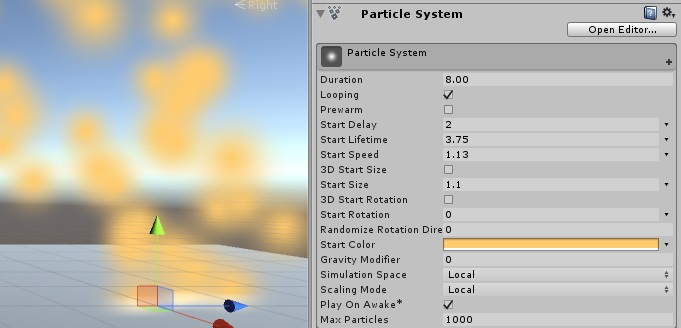
\includegraphics[width=0.95\linewidth]{Abbildungen/Unity/Fire/fire1}
\caption{Grundeinstellung Partikelsystem}
\label{fig:fire1}
\end{figure}

Im ersten Schritt wird ein Gameobject \textit{Particle System} erstellt und die in Abb. \ref{fig:fire1} abgebildeten Grundeinstellungen vorgenommen.

\begin{figure}[h!]
\centering
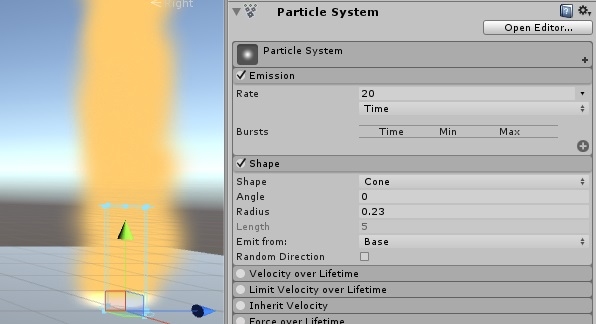
\includegraphics[width=0.95\linewidth]{Abbildungen/Unity/Fire/fire2}
\caption{Einstellungen Emission und Shape}
\label{fig:fire2}
\end{figure}

Um die Partikel zu verdichten und die horizontale Streuung einzugrenzen, wird die Emission erhöht und die Form angepasst. (siehe Abb.\ref{fig:fire2}) 

\begin{figure}[h!]
\centering
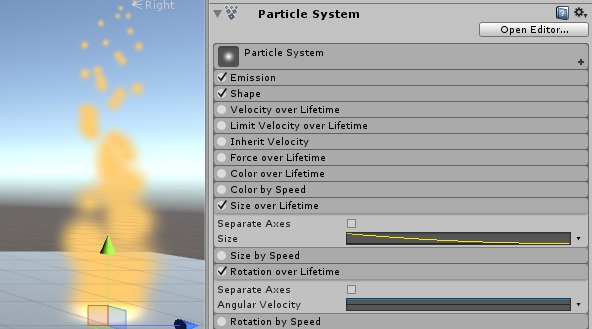
\includegraphics[width=0.95\linewidth]{Abbildungen/Unity/Fire/fire3}
\caption{Einstellungen Size over Livetime und Rotation over Lifetime}
\label{fig:fire3}
\end{figure}

Die typische Flammenform erreicht man, indem man die Größe im Bezug zur Lebensdauer anpasst. Dazu wählt man eine exponentiell sinkende Kurve. Außerdem versetzt man die Partikel in eine Rotation. (siehe Abb. \textit{fire3})

\begin{figure}[h!]
\centering
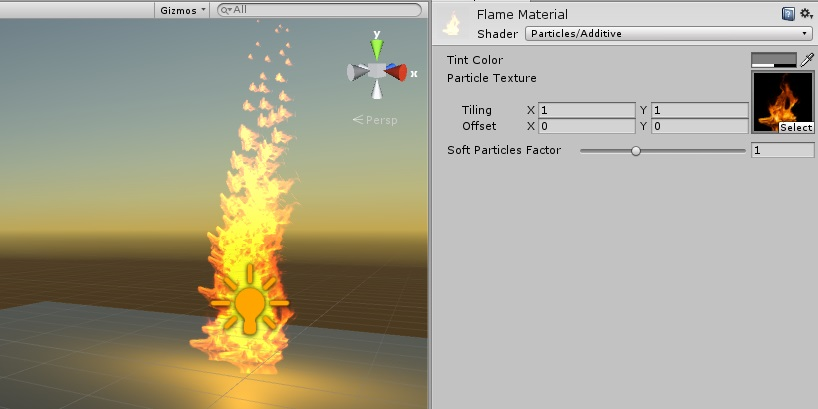
\includegraphics[width=0.95\linewidth]{Abbildungen/Unity/Fire/fire4}
\caption{Material und Point Light}
\label{fig:fire4}
\end{figure}

Um einen Flammenähnlichen Farbverlauf zu erreichen, muss man dem Partikelsystem ein Material zufügen. Dieses besteht aus dem Bild einer Flame auf schwarzem Hintergrund und entfaltet durch den Shader \textit{Particles/Additive} den gewünschten Effekt.

\newpage

\subsection{Benutzeroberfläche}
\subsubsection{Hauptmenü}
\subsubsection{}






 

